\chapter{Ogólna koncepcja i architektura}

Aplikacja \emph{TeamSync} zrealizowana w ramach niniejszej pracy ma strukturę dwuwarstwową. Strony serwera oraz klienta, na wzór serwisów internetowych, są od siebie odizolowane, a komunikacja między nimi zachodzi z wykorzystaniem protokołu \texttt{HTTP} \cite{http} \cite{httparticle}. BitTorrent Sync jest narzędziem współpracującym z aplikacją, które jest odpowiedzialne za wymianę danych (synchronizację). Komunikacja z tym narzędziem jest możliwa dzięki odpowiednio skonfigurowanemu API, które zostało udostępnione przez twórców całego systemu.

Działanie aplikacji \emph{TeamSync} polega na uruchomieniu w tle systemu synchronizującego dane i udostępnienie użytkownikowi wygodnego interfejsu do umieszczania i odczytywania komentarzy, co odbywa się poprzez odpowiednią manipulację plikami wewnątrz synchronizowanych folderów. Jedyną drogą wymiany danych jest wspomniany system BitTorrent Sync.

\begin{figure}[htb]
  \vspace{5pt}
  \begin{center}
    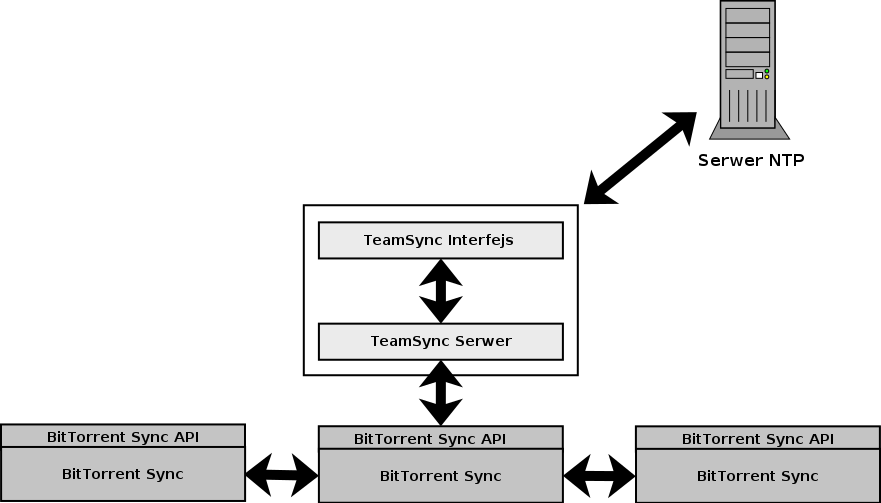
\includegraphics[width=380pt]{figures/architecture3.png}
  \end{center}
  \caption{Uproszczona architektura systemu \emph{TeamSync}.}
  \label{architecturepic}
\end{figure}

Poniżej zostaną omówione w oddzielnych podrozdziałach poszczególne moduły architektury systemu: BitTorrent Sync, system \emph{TeamSync} wraz z komunikacją pomiędzy jego częścią serwerową a kliencką oraz serwer NTP.

\section{BitTorrent Sync}

W poniższej sekcji opisanych zostanie kilka aspektów zarówno systemu BitTorrent Sync, jak i zaimplementowanemu przez jego twórców API, dzięki któremu możliwe jest wykonywanie większości funcji tego systemu z poziomu kodu. Rozdział rozpocznie sekcja \emph{secret} opisująca łańcuch znaków wymieniany między użytkownikami, po której zostanie przedstawiony bardziej szczegółowy opis protokołu komunikacji z systemem BitTorrent Sync.

\subsection{Secret}

\label{secret}

W aplikacji BitTorrent Sync \emph{secret} jest ciągiem $32$ znaków, służącym do identyfikacji synchronizowanych folderów. Dodając katalog do tego systemu, użytkownik może posłużyć się istniejącym już \emph{secretem}, jeśli otrzymał go od użytkownika, który wcześniej zainicjował folder. Może też sam go zainicjować, generując \emph{secret} tworząc losowy ciąg znaków odpowiadający wyrażeniu regularnemu \texttt{[A-Z0-9]\{32\}}, co odpowiada trzydziestu dwóm losowym znakom wybranym ze zbioru cyfr od $0$ do $9$ oraz liter alfabetu od \texttt{A} do \texttt{Z}.

Duża ilość znaków ($32$ znaki) oraz duży ich zbiór ($24$ litery $+$ $10$ cyfr daje łącznie moc zbioru znaków równą $34$) powodują, że istnieje znikoma szansa na powtórzenie się dwóch łańcuchów znakowych.

Podczas generowania wartości \emph{secret}, tworzone są dwa łańcuchy znaków o dwóch typach synchronizacji:

\begin{description}[noitemsep]
  \item[read\_write] --- użytkownicy, którzy otrzymają \emph{secret} pochodzący z tej wartości będą mogli zarówno odczytywać dane, jak i je modyfikować oraz dodawać swoje; modyfikacje danych --- w przeciwieństwie do trybu \texttt{read\_only} --- będą się propagować do pozostałych użytkowników,
  
  \item[read\_only] --- użytkownicy, którzy otrzymają ten \emph{secret}, będą mogli wyłącznie pobierać dane, nie mogąc ich modyfikować (niezależnie od modyfikacji, zmiany nie będą propagowane do innych użytkowników).
\end{description}

W zależności od tego, który z \emph{secretów} użytkownik otrzyma, tak system będzie uspójniał dane.

\subsection{Protokół BitTorrent Sync API}

\label{btsyncapiproto}

Twórcy systemu BitTorrent Sync umożliwili korzystanie z dodatkowej funkcjonalności aplikacji nie tylko użytkownikom, ale również programistom chcącym testować lub udoskonalać narzędzia związane z wymianą plików. Sterowanie systemem z poziomu kodu jest możliwe dzięki zaimplementowanemu przez twórców aplikacji API, które umożliwia komunikację pomiędzy narzędziem a stworzoną przez programistę aplikacją.

API narzędzia odbiera żądania --- z odpowiednio dobranymi parametrami --- nasłuchując na porcie wskazanym przez użytkownika w pliku konfiguracyjnym (dokładny opis pliku konfiguracyjnego znajduje się w podrozdziale \ref{configbtsync}). Pełen adres, na który programista musi skierować żądanie HTTP ma postać wzorca:
\begin{verbatim}
                          http://<adres>:<port>/api
\end{verbatim}

W przypadku aplikacji \emph{TeamSync} zaimplementowanej w ramach niniejszej pracy magisterskiej, ze względu na lokalizację systemu BitTorrent Sync (lokalna maszyna) użyty adres to \texttt{localhost} oraz port \texttt{8787} (zmieniony z domyślnego \texttt{8888} ze względu na jego dużą popularność w aplikacjach). Pełen adres, na który są wysyłane żądania pomiędzy aplikacją \emph{TeamSync}, a API systemu BitTorrent Sync to:
\begin{verbatim}
                          http://localhost:8787/api
\end{verbatim}

\subsubsection*{Komunikaty BitTorrent Sync API}

Żądania wysyłane z systemu \emph{TeamSync} do API zawierają w nagłówku parametr uwierzytelniający \emph{Basic HTTP Authentication} \cite{basicauth}. Dane dostępu zawierają wartości \texttt{login} oraz \texttt{password}, które --- aby zostały poprawnie odebrane --- muszą odpowiadać danym umieszczonym wewnątrz pliku konfiguracyjnego systemu BitTorrent Sync. Uruchamiając po raz pierwszy aplikację \emph{TeamSync} dane uwierzytelniające są tworzone wraz z plikami konfiguracyjnymi i ustawione domyślnie na \texttt{team} oraz \texttt{sync} odpowiednio dla wartości \texttt{login} oraz \texttt{password}.

Zapytania przyjmowane przez BitTorrent Sync API zawierają dodatkowo tzw. ,,metodę'' wraz z jej argumentami. Metoda oznacza funkcję, która zostanie wykonana na podanych argumentach np. pobieranie listy folderów wprowadzonych do systemu i współdzielonych z innymi użytkownikami, pobieranie listy użytkowników, z którymi użytkownik synchronizuje dany folder, zwrócenie ustawień konkretnego folderu lub ich zmiana i wiele innych. W aplikacji \emph{TeamSync} użyto niewielkiej ilości możliwych metod ze względu na ich dużą liczebność i użyteczność odbiegającą od głównego celu projektu.

Użyte metody wraz z typem przyjmowanych argumentów zostaną opisane w oddzielnych sekcjach. Wszystkie zwroty użyte w poniższych podrozdziałach dotyczące aplikacji takie jak: ,,aplikacja'', ,,system'', ,,narzędzie'', będą dotyczyły systemu BitTorrent Sync. Sposób działania narzędzia zaimplementowanego w ramach niniejszej pracy nie będzie omawiany podczas opisu poniższych metod.

Przykłady dotyczące sposobu wysyłania zapytań przez aplikację \emph{TeamSync} są napisane według wzoru podyktowanego przez wymagania funkcji pakietu \texttt{requests} języka \emph{Python}, które zostały użyte do wysyłania żądań do BitTorrent Sync API.

\begin{minipage}{\linewidth}
\vspace{15pt}
\begin{verbatim}
            requests.get('http://adres:port/api',
                         auth=('login', 'password'),
                         params={
                             'method': 'nazwa_metody',
                             'arg1': 'wartość_argumentu',
                             [ . . . ]
                         }
            )
\end{verbatim}
\vspace{15pt}
\end{minipage}

Pierwszy argument wewnątrz zapytania reprezentuje adres wraz z numerem portu, na który zostanie wysłane żądanie. Dane uwierzytelniające przesyłane są wewnątrz parametru \texttt{auth}, natomiast nazwa metody oraz pozostałe argumenty przesyłane są wewnątrz parametru \texttt{params}, który ma strukturę słownika z nazwą oraz wartością poszczególnych argumentów.

\subsubsection*{\emph{get\_secrets}}

\label{getsecrets}

Metoda \emph{get\_secrets} nie wymaga żadnych dodatkowych argumentów i służy do generowania przez aplikację ciągów znakowych identyfikujących synchronizowany folder.  Zapytanie wysyłane do BitTorrent Sync API w celu ich uzyskania:

\begin{minipage}{\linewidth}
\vspace{15pt}
\begin{verbatim}
               requests.get('http://localhost:8787/api',
                            auth=('team', 'sync'),
                            params={
                                'method': 'get_secrets',
                            }
               )
\end{verbatim}
\vspace{15pt}
\end{minipage}

Odpowiedź aplikacji będąca słownikiem w formacie \texttt{JSON} \cite{jsonarticle} zawiera dwie wartości:

\begin{itemize}[noitemsep]
  \item \emph{read\_write} --- \emph{secret} służący do synchronizacji folderu w trybie zapisu/odczytu,
  \item \emph{read\_only} --- \emph{secret}, za pomocą którego użytkownik może udostępnić swoje dane, nie pozwalając na modyfikację lub dodawanie danych innym użytkownikom.
\end{itemize}

\subsubsection*{\emph{add\_folder}}

Metoda dodająca wskazany w argumencie folder do systemu. Po otrzymaniu żądania zawierającego tę metodę, do wybranego katalogu --- który w momencie wykonywania metody musi być pusty (wymaganie systemu BitTorrent Sync) --- aplikacja dodaje ukryty folder \texttt{.sync} (dokładny opis zawartości katalogu \texttt{.sync} znajduje się w podrozdziale \ref{directorystructure}) i od tego momentu katalog wskazany w żądaniu będzie włączony do synchronizacji.

Oprócz metody komunikat zawiera dodatkowe parametry:

\begin{itemize}[noitemsep]
  \item \emph{dir} --- pełna ścieżka do folderu,
  \item \emph{secret} --- losowy ciąg znaków będący tzw. ,,secretem'', za pomocą którego możliwa jest synchronizacja katalogów między użytkownikami. Jeśli parametr ten pozostanie pusty, system otrzyma informację, że folder jest nowy i nie jest jeszcze synchronizowany przez żadnego z użytkowników. Aplikacja wygeneruje secret i od tego momentu użytkownik może przekazywać go innym węzłom, aby współdzielić wskazany katalog.
\end{itemize}

Zakładając, że synchronizowany ma zostać katalog o ścieżce \texttt{/home/user/testowy\_katalog}, zapytanie zostanie wysłane z serwera aplikacji \emph{TeamSync} w następujący sposób:

\begin{minipage}{\linewidth}
\vspace{15pt}
\begin{verbatim}
     requests.get('http://localhost:8787/api',
                  auth=('team', 'sync'),
                  params={
                      'method': 'add_folder',
                      'dir': '/home/user/testowy_katalog',
                      'secret': 'A3LL43HJ257YCKMOLAD7QSEAS7U373BVO'
                  }
     )
\end{verbatim}
\vspace{15pt}
\end{minipage}

W przypadku otrzymania takiego komunikatu z pustym argumentem \texttt{secret}, aplikacja wygenerowałaby nowy secret i zwróciłaby go w odpowiedzi. W innym przypadku, w odpowiedzi przesyłany jest wyłącznie kod błędu wewnątrz zmiennej \texttt{error}. W przypadku otrzymanej wartości równej $0$ użytkownik jest informowany, że operacja dodawania nowego folderu przebiegła pomyślnie.

\subsubsection*{\emph{get\_folders}}

Za pomocą tej metody otrzymywana jest lista folderów, które zostały wprowadzone do systemu. Podobnie jak przy metodzie \emph{get\_secrets} żadne dodatkowe argumenty nie są wymagane.

\begin{minipage}{\linewidth}
\vspace{15pt}
\begin{verbatim}
               requests.get('http://localhost:8787/api',
                            auth=('team', 'sync'),
                            params={
                                'method': 'get_folders',
                            }
               )
\end{verbatim}
\vspace{15pt}
\end{minipage}

W odpowiedzi na zapytanie \emph{get\_folders} BitTorrent Sync API zwraca listę, wewnątrz której znajdują się informacje o wszystkich synchronizowanych w systemie folderach w formacie \texttt{JSON}. Wśród kluczy słowników są:

\begin{itemize}[noitemsep]
  \item \emph{error} --- w przypadku niepowodzenia przesyłana jest tylko ta wartość ustawiona na $1$; w przypadku powodzenia wartość $0$,
  
  \item \emph{dir} --- bezwzględna ścieżka folderu w systemie plików lokalnego użytkownika,
  
  \item \emph{files} --- liczba plików, które znajdują się wewnątrz folderu,
  
  \item \emph{size} --- łączny rozmiar plików wewnątrz folderu w bajtach,
  
  \item \emph{secret} --- łańcuch znaków służący do identyfikacji współdzielonych folderów między zdalnymi użytkownikami (więcej w sekcji \ref{secret}),
  
  \item \emph{type} --- rodzaj synchronizacji; możliwe dwie wartości:
  \begin{itemize}[noitemsep]
    \item \emph{read\_write} --- użytkownicy mogą zarówno odczytywać, jak i modyfikować pliki,
    
    \item \emph{read\_only} --- tylko właściciel może modyfikować, pozostali użytkownicy wyłącznie odczytywać,
  \end{itemize}
  
  \item \emph{down\_speed} --- chwilowa prędkość pobierania; jeśli wszystkie dane w folderze są zsynchronizowane, wartość $0$,
  
  \item \emph{up\_speed} --- chwilowa prędkość wysyłania; jeśli wszystkie dane w folderze są zsynchronizowane, wartość $0$,
  
  \item \emph{id} --- unikalny identyfikator folderu, który może różnić się pomiędzy użytkownikami.
\end{itemize}

Przykładowa odpowiedź BitTorrent Sync API na powyższe żądanie może wyglądać następująco:

\begin{minipage}{\linewidth}
\vspace{15pt}
\begin{verbatim}
         [
             {
                 "error": 0, 
                 "dir": "/home/user/testowy katalog", 
                 "files": 9, 
                 "size": 3079, 
                 "secret": "A3LL43HJ257YCKMOLAD7QSEAS7U373BVO", 
                 "type": "read_write", 
                 "down_speed": 0, 
                 "up_speed": 0, 
                 "id": 902958156496830188
             }
         ]
\end{verbatim}
\vspace{15pt}
\end{minipage}

Otrzymanie takiej odpowiedzi wskazuje na fakt, iż jednym (i jedynym, ze względu na obecność tylko jednego obiektu typu \texttt{JSON} w liście katalogów) z synchronizowanych folderów w systemie jest folder o ścieżce \texttt{/home/user\-/testowy katalog}. Został on poprawnie odczytany przez system BitTorrent Sync (\texttt{'error': 0}) i zawiera dziewięć plików o łącznym rozmiarze $3079$ bajtów. Aby uwspólnić go z innymi użytkownikami w trybie umożliwiającym im zarówno odczyt, jak i modyfikację zawartości (tryb \texttt{read\_write}), należy przekazać \emph{secret} o wartości \texttt{A3LL43HJ\-257YCKMO\-LAD7QSEAS\-7U373BVO}.

Wartości \texttt{down\_speed} oraz \texttt{up\_speed} sugerują brak wymiany danych między użytkownikami w chwili wysyłania żądania \emph{get\_folders}. Wewnętrznym identyfikatorem folderu w systemie lokalnym użytkownika jest liczba \texttt{902958156496830188}.

\subsubsection*{remove\_folder}

Ostatnią z używanych przez system \emph{TeamSync} metod jest metoda \emph{remove\_folder}, która usuwa z systemu wskazany synchronizowany folder --- nie usuwa fizycznie katalogu z systemu plików, lecz blokuje jego dalszą synchronizację. Aby ponownie użyć tego samego katalogu, należy usunąć z niego wszystkie pliki (wymaganie aplikacji dotyczące pustego folderu). W parametrze żądania --- oprócz metody --- aplikacja potrzebuje wartość \emph{secret} folderu, który użytkownik zamierza usunąć.

\begin{minipage}{\linewidth}
\vspace{15pt}
\begin{verbatim}
       requests.get('http://localhost:8787/api',
                    auth=('team', 'sync'),
                    params={
                        'method': 'remove_folder',
                        'secret': 'A3LL43HJ257YCKMOLAD7QSEAS7U373BVO'
                    }
       )
\end{verbatim}
\vspace{15pt}
\end{minipage}

W przeciwieństwie do metody \emph{add\_folder}, w której parametr \emph{secret} był opcjonalny, tutaj konieczne jest przesłanie tego parametru. Jeśli nie zostanie on przesłany lub okaże się niepoprawny, aplikacja zwróci kod błędu w zmiennej \texttt{error}. W przypadku poprawnego przebiegu operacji \emph{remove\_folder}, kod błędu będzie równy $0$.

\section{\emph{TeamSync}}

\label{teamsyncarch}

Po opisaniu modułu BitTorrent Sync API z Rys. \ref{architecturepic} umieszczonego no początku rozdziału, przedstawiony zostanie dokładniej sposób działania systemu \emph{TeamSync} --- jak zapisywane są komentarze oraz wątki, jak są przekazywane w sieci oraz w jaki sposób system unika konfliktów.

\subsection{Komentarze}

\label{archcomments}

Rozproszona architektura nie daje pewności, że modyfikacja pliku odbędzie się bezkonfliktowo, ponieważ zawsze może wystąpić sytuacja, w której inny węzeł ,,równocześnie'' (pod względem zegara logicznego, nie czasu rzeczywistego) nie dokona edycji danych. Podczas testów aplikacji BitTorrent Sync, która jest odpowiedzialna za wymianę danych --- a więc również za rozwiązywanie konfliktów --- nie wyizolowano priorytetów określających, którą wersję i z którego węzła należy usunąć, a z którego rozpropagować.
 
Z powyżej opisanych powodów umieszczanie komentarzy w aplikacji \emph{TeamSync} polega na \emph{dodawaniu} nowych plików przez użytkowników. Algorytm dodawania nowego komentarza z lokalnej perspektywy wygląda następująco:

\begin{enumerate}[noitemsep]
 \item Pobierz znacznik czasowy z serwera NTP.
 
 \item Umieść pobrane od użytkownika dane (treść komentarza, identyfikator) oraz pobrany wcześniej znacznik czasowy do zmiennej o strukturze słownika (JSON).
 
 \item Zapisz słownik do pliku o nazwie złożonej ze znacznika czasowego oraz identyfikatora użytkownika wewnątrz katalogu z wątkiem.
\end{enumerate}

Umieszczenie komentarza w systemie i rozpropagowanie go pomiędzy wszystkich aktywnych użytkowników zaprezentowane jest na rysunku \ref{rys:writecomment}.

\begin{figure}[t]
  \vspace{5pt}
  \begin{center}
    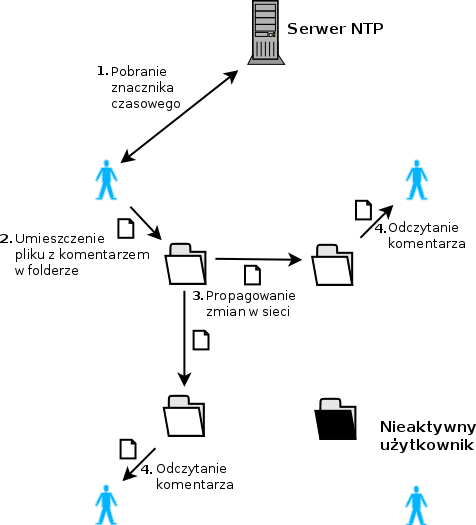
\includegraphics[width=220pt]{figures/writecomment.png}
  \end{center}
  \caption{Uproszczony schemat dodawania nowego komentarza do systemu i odczytanie go przez aktywnych użytkowników.}
  \label{rys:writecomment}
\end{figure}

\subsubsection*{Struktura komentarzy}

Wszystkie zapisywane komentarze mają swoją strukturę, która --- podobnie jak w przypadku wszystkich danych przesyłanych i zapisywanych do plików w aplikacji \emph{TeamSync} --- jest strukturą słownikową zapisaną w formacie JSON. Każdy plik komentarza zawiera pięć kluczy wraz z wartościami:

\begin{itemize}[noitemsep]
 \item \emph{comment} --- treść komentarza,
 
 \item \emph{timestamp} --- znacznik czasowy pobierany podczas powstawania komentarza,
 
 \item \emph{history} --- lista zawierająca obiekty o strukturze słownikowej, które przechowują wszelkie zmiany treści komentarza w wartościach kluczy \texttt{comment} oraz \texttt{timestamp}. W momencie zmiany treści przez autora wypowiedzi, dodawany jest nowy element w liście \texttt{history} z obiektem o tych kluczach z wartościami wypełnionymi nową treścią (\texttt{comment}) oraz nowym znacznikiem czasowym (\texttt{timestamp}),
 
 \item \emph{uid} --- autor komentarza,
 
 \item \emph{readby} --- zmienna o strukturze słownika przechowująca informację o użytkownikach, którzy odczytali komentarz i o czasie, w którym to zrobili. W kluczu znajduje się identyfikator autora, natomiast jako wartość wpisywany jest znacznik czasowy odczytania posta.
\end{itemize}

Po zatwierdzeniu zmiany wyświetlana jest najnowsza treść komentarza, natomiast znacznik czasowy pozostaje bez zmian. Taka implementacja jest wymuszona przez konieczność zachowania ciągłości logicznej konwersacji --- edytowany post nie może przemieszczać się w chronologicznym porządku wymiany opinii, ponieważ część wypowiedzi może zostać źle odczytana w przypadku modyfikacji komentarzy przed nią. Intencje edycji zazwyczaj polegają na korygowaniu napisanych wcześniej zdań (interpunkcja, ,,literówki'', ortografia) lub dodawaniu mniej znaczących faktów --- rzadko zdarza się całkowita modyfikacja treści, a w przypadku gdy jednak wystąpi, użytkownicy mogą przejrzeć historię komentarzy, gdy dostrzegą logiczne niezgodności w przepływie opinii.

\subsubsection*{Konflikty}

Struktura pliku z komentarzem może być bardzo dynamiczna i często zmieniana, ponieważ istnieje lista (\texttt{history}), w której dodawane sa elementy, oraz słownik (\texttt{readby}) uzupełniany o kolejne pary klucz-wartość. Czy wobec tego nie generuje to konfliktów, które mogłyby naruszyć spójność danych? Czy użytkownik \texttt{A} może znaleźć się w sytuacji, że ,,ominie'' go część informacji, gdy użytkownik \texttt{B} nadpisze swoją część zamiast części użytkownika \texttt{C}? Lub czy jest możliwość, że modyfikacja użytkownika \texttt{A} zostanie pominięta, ponieważ w tym samym czasie użytkownik \texttt{B} dokonał zmian w tym samym komentarzu i ,,wygrał'' synchronizację?

Odpowiedź brzmi: TAK, jest taka możliwość.

Modyfikacja komentarzy zachodzi w dwóch przypadkach: edycji treści oraz odczytaniu go przez użytkownika. Poniżej zostaną rozważone obydwa przypadki i w każdym z nich opisane zostaną możliwości konfliktów oraz ich skutki.

\begin{description}[noitemsep]
  \item[Modyfikacja treści] --- wystąpienie konfliktu w przypadku edytowania treści jest niemożliwe, ponieważ interfejs użytkownika pozwala na poprawienie treści tylko w przypadku, gdy jesteś autorem komentarza. Jeden użytkownik nie jest w stanie dokonać edycji dwóch postów jednocześnie.
  
  \item[Odznaczenie jako przeczytane] --- w tym przypadku konflikt może wystąpić, lecz nie będzie miał żadnych poważnych konsekwencji. Żeby to wyjaśnić, załóżmy, że użytkownicy \texttt{A} oraz \texttt{B} nie przeczytali jeszcze pewnego komentarza \texttt{x} i zrobią to w tym samym momencie (albo każdy z nich zrobi to na swojej lokalnej wersji, gdy żaden z pozostałych użytkowników należących do folderu nie będzie dostępny). W obecnej chwili (przed wzajemną synchronizacją) obydwaj użytkownicy mają oznaczony post \texttt{x} jako przeczytany. W momencie synchronizacji ,,wygra'' wersja pliku któregoś z użytkowników. Załóżmy, że wygra użytkownik \texttt{A}: wówczas użytkownik \texttt{B} zobaczy w swojej aplikacji \emph{TeamSync}, że ponownie ma nieprzeczytany komentarz, ale wówczas znowu aplikacja ,,przeczyta'' komentarz ponownie odpowiednio go modyfikując (wstawiając nową parę klucz-wartość do słownika \texttt{readby}).
  
  Nawet w przypadku częstych konfliktów, wpływa to nieznacznie tylko i wyłącznie na wygodę użytkownika (ponowne ,,kliknięcie'' na nieprzeczytany wątek).
\end{description}

\subsubsection*{Przykładowy komentarz}

Na rysunku \ref{rys:comment} przedstawiona została struktura komentarza, który dla lepszego zobrazowania własnej struktury został odczytany przez trzech użytkowników i był modyfikowany dwukrotnie.

\begin{figure}[t]
  \label{rys:comment}
  \begin{verbatim}
            {
                "comment": "Ostateczna treść komentarza", 
                "timestamp": "1439395604000", 
                "history": [
                    {
                        "comment": "Pierwsza treść", 
                        "timestamp": "1439395604000"
                    },
                    {
                        "comment": "Pierwsza treść zmodyfikowana", 
                        "timestamp": "1439395945000"
                    },
                    {
                        "comment": "Ostateczna treść komentarza", 
                        "timestamp": "1439396291000"
                    }
                ], 
                "uid": "2HI7KRUNSSONIUJKMRWXGOTIZSHBGFIH", 
                "readby": {
                    "2HI7KRUNSSONIUJKMRWXGOTIZSHBGFIH": "1439395604000",
                    "2SAFDSBCXGFD765GDFS4GFDS35FDSBVB": "1439395888000",
                    "3REW54GFDS6578FDSGDF5BSH652F2B34": "1439396782000"
                }
            }
  \end{verbatim}
  \caption{Struktura przykładowego komentarza.}
\end{figure}

W poniższym przykładzie dobrze widać zmianę treści komentarza poprzez pobranie jej z najświeższej modyfikacji oraz niezmienność znacznika czasowego (\texttt{timestamp}) niezależnie od tego, czy komentarz był modyfikowany. Zauważalna jest też łatwość, z jaką można odtworzyć całą historię zmian wypowiedzi. Oglądanie zmian wszystkich komentarzy jest dostępne dla każdego z użytkowników niezależnie od przynależności, o ile taka historia dla konkretnego przypadku istnieje.

Dzięki słownikowi \texttt{readby} można odczytać, który z użytkowników i w jakim czasie odczytał ten komentarz: na przykład użytkownik o identyfikatorze \texttt{2HI7KRUN\-SSONIUJ\-KMRWXGOTI\-ZSHBGFIH} podczas odczytywania wypowiedzi umieścił swój wpis, pobierając znacznik czasowy \texttt{1439395604000}, co odpowiada dacie \texttt{12.08.2015r.} i godzinie \texttt{18:06} czasu polskiego.

\subsection{Wątki}

Wewnątrz każdego folderu z wątkiem oprócz plików z komentarzami znajduje się plik o nazwie \texttt{meta}, który zawiera dane związane z wątkiem prezentowane w interfejsie użytkownika. Podobnie jak w przypadku komentarzy, są one ustrukturyzowane jako para klucz/wartość w formacie JSON. Klucze znajdujące się w pliku \texttt{meta} obejmują następujące informacje:

\begin{itemize}[noitemsep]
  \item \emph{uid} --- autor wątku,
  \item \emph{timestamp} --- znacznik czasowy pobrany podczas tworzenia wątku (identyczny ze znacznikiem czasowym pierwszego komentarza),
  \item \emph{fileabout} --- ścieżka wewnątrz folderu wskazująca na plik, którego dotyczy watek,
  \item \emph{topic} --- tytuł watku.
\end{itemize}

Plik \texttt{meta} został wprowadzony w celu szybszego odczytywania listy wątków --- podczas przygotowywania listy, odczytywanie przez aplikację komentarzy jest niepotrzebne, dzięki czemu aplikacja działa szybciej. Pobieranie komentarzy z folderu zawierającego wątek (treści, znaczników czasowych itd.) następuje \emph{po} wybraniu konkretnej dyskusji.

Informacje dodatkowe wątku (np. ilość napisanych komentarzy, znacznik czasowy najświeższego komentarza) są na bieżąco obliczane przez aplikację podczas pobierania listy wątków. Znaczniej łatwiej (oraz szybciej) byłoby zapisać te dane w pliku \texttt{meta} i odczytywać je z otwartego już pliku. Natomiast wówczas pojawiłaby się możliwość wystąpienia konfliktów podczas jego edycji. Węzeł, który dodawałby nowy komentarz, musiałby edytować plik \texttt{meta} i inkrementować licznik komentarzy oraz zmodyfikować czas najświeższego komentarza. W przypadku dwóch użytkowników dodających komentarz w tym samym czasie dochodziłoby do konfliktów i umieszczania fałszywych danych wewnątrz pliku.

Dwie z informacji o wątku --- autor oraz znacznik czasowy --- są powielone z pierwszego komentarza w dyskusji (ponieważ podczas zakładania wątku umieszczany jest również inicjujący go komentarz). Zaimplementowano to w taki sposób, aby mieć dostęp do danych o wątku bez konieczności odczytywania któregokolwiek z komentarzy (np. odczytanie pierwszego komentarza wymaga sortowania, ponieważ funkcja modułu \texttt{os} języka \emph{Python} o nazwie \texttt{listdir} listuje nieuporządkowaną zawartość katalogu przyjmowanego w argumencie.

\subsubsection*{Przykładowy plik \texttt{meta}}

Poniżej przedstawiony został przykładowy plik z metadanymi wątku o nazwie ,,Przykładowy wątek''.

\begin{figure}[htb]
  \label{thread}
  \begin{verbatim}
                  {
                      "topic": "Przykładowy wątek", 
                      "timestamp": "1439395604000", 
                      "fileabout": "/katalog1/test.txt",
                      "uid": "2HI7KRUNSSONIUJKMRWXGOTIZSHBGFIH", 
                  }
  \end{verbatim}
  \caption{Struktura przykładowego pliku z metadanymi wątku.}
\end{figure}

Według tego przykładowego pliku wątek został utworzony --- zgodnie ze znacznikiem czasowym --- 30. sierpnia 2015 r. o godzinie \texttt{9:23}. Autorem jest użytkownik o identyfikatorze \texttt{2HI7KRU\-NSSONIUJ\-KMRWXGOTI\-ZSHBGFIH}. Dyskusja o tytule ,,Przykładowy wątek'' rozpoczęta przez tego użytkownika dotyczy pliku \texttt{test.txt}, który znajduje się wewnątrz folderu \texttt{katalog1} wewnątrz folderu synchronizowanego.

Strukturę przykładowego synchronizowanego folderu --- zawierający zarówno wątek z powyższego przykładu jak i plik opisywany w dyskusji --- przedstawiono poniżej:

\begin{minipage}{\linewidth}
\vspace{1em}
\begin{verbatim}
    [root]/
        .sync/
            [ pliki aplikacji BitTorrent Sync ]
        .Users/
            [ pliki z danymi o użytkownikach ]
        .Comments/
            katalog1/
                1439395604000@#&$Przykładowy wątek/
                    meta
                    1439395604000@#&$2HI7KRUNSSONIUJKMRWXGOTIZSHBGFIH
            1439423576000@#&$Inny wątek/
                meta
                1439423576000@#&$2SAFDSBCXGFD765GDFS4GFDS35FDSBVB
                1439476598000@#&$2HI7KRUNSSONIUJKMRWXGOTIZSHBGFIH
        katalog1/
            test.txt
            ccc.txt
        aaa.txt
        bbb.txt
\end{verbatim}
\vspace{1em}
\end{minipage}

Widać wewnątrz poniższej struktury, że ,,Przykładowy wątek'' został umieszczony w folderze \texttt{.Comments} w lokalizacji takiej samej, jak oryginalny plik, o którym powstała dyskusja (\texttt{katalog1}). Wewnątrz niego znajduje się plik z metadanymi o wcześniej przedstawionej strukturze oraz jeden komentarz. Warto zauważyć, że w nazwie komentarza jest ten sam znacznik czasowy, który jest zapisany w pliku \texttt{meta} --- według zasad opisanych wcześniej.

W przykładzie umieszczono również drugi wątek, zlokalizowany najpłycej w katalogu \texttt{.Comments}. Oznacza to, że w interfejsie graficznym będzie on wylistowany zawsze, gdy użytkownik nawigując po folderze, będzie przebywał na najwyższym jego poziomie --- ,,korzeniu''. ,,Inny wątek'' --- bo tak należy odczytać tytuł tej dyskusji, zawiera dwa komentarze --- jeden napisany przez użytkownika \texttt{2SAFDSB\-CXGFD765\-GDFS4GFDS\-35FDSBVB} w chwili pobrania znacznika czasowego \texttt{1439423\-576000} oraz przez użytkownika \texttt{2HI7KRU\-NSSONIUJ\-KMRWXGO\-TIZSHBGFIH} w chwili \texttt{1439476\-598000}.

\subsection{Nazwy folderów i plików}

\label{filenamesf}

Foldery zawierające wątki oraz pliki z komentarzami są tworzone przez dowolny węzeł w dowolnym czasie, co zwiększa niebezpieczeństwo wystąpienia konfliktów w nazwach tworzonych plików za każdym razem, gdy użytkownik wypowiada się w dyskusji lub rozpoczyna nową. Dodatkowo drzewiasta struktura katalogu \texttt{.Comments}, wewnątrz którego przechowywane są komentarze, powoduje, że ,,zwykłe'' foldery przechowywane są obok katalogów zawierających pliki komentarzy. Przeszukiwanie ich wszystkich przez serwer poprzez przeglądanie wszystkich lokalizacji jest wolniejsze i przy folderze mocno rozbudowanym systemem katalogów może odczuwalnie spowolnić aplikację.

Mając na uwadze powyższe problemy, projektując aplikację \emph{TeamSync} przyjęto następujące dwie zasady --- dotyczące nazw zarówno plików komentarzy, jak i folderów z wątkami --- jako konieczne do spełnienia. Konsekwencje nieprzestrzegania każdej z zasad będą wyjaśnione w dalszej części sekcji.

\begin{enumerate}[noitemsep]
  \item System powinien uniemożliwiać (zapewniać poziom prawdopodobieństwa \emph{w praktyce} uniemożliwiający) powtarzanie się \emph{nazwy} pliku komentarza lub folderu wątku.
  
  \item Nazwy powinny zawierać w sobie pewien element (ciąg znaków), dzięki któremu serwer odczyta informację, że wybrany folder lub plik to odpowiednio folder zawierający wątek oraz plik przechowujący wypowiedź. Informacja o wyjątkowości katalogu musi być zawarta w jego nazwie.
\end{enumerate}

Opisy sposobów realizacji obydwóch zasad zostały opisane w poniższych podrozdziałach.

\subsubsection*{Unikalność nazwy}

Jeśli w przypadku plików z komentarzami unikalność wprowadzanych nazw nie byłaby zachowana, efektem byłby konflikt skutkujący nadpisaniem pliku. Użytkownik \texttt{A} zatwierdzający treść odpowiedzi umieściłby swój plik, który chwilę później byłby nadpisany przez użytkownika \texttt{B}. Wersja użytkownika \texttt{A} zostałaby uznana jako nieaktualna i w konsekwencji przeniesiona do katalogu \texttt{Archive} w ukrytym folderze \texttt{.sync}, do którego użytkownicy nie mają dostępu z poziomu aplikacji \emph{TeamSync}.

Podobnie --- lecz z innymi konsekwencjami --- wygląda sytuacja w przypadku tworzenia nowego wątku. Gdyby ten sam użytkownik \texttt{A} tworzył nowy wątek w tym samym momencie, co użytkownik \texttt{B}, również wystąpiłby konflikt, lecz z odmiennymi skutkami. W kodzie serwera zastosowano instrukcję warunkową przed tworzeniem nowego folderu wątku sprawdzającą, czy taki folder już istnieje. Aplikacja tworzy nowy katalog, jeśli jeszcze nie istniał wcześniej w systemie plików --- w odwrotnym przypadku serwer kontynuuje działanie bez żadnych zmian. Efektem konfliktu byłoby nienadpisanie folderu z wątkiem, a nadpisanie pliku \texttt{meta} oraz (w zależności czy unikalność nazwy pliku z komentarzem została zachowana) możliwość nadpisania lub dodania nadmiarowego komentarza. W obecnym przypadku (użytkownicy \texttt{A} oraz \texttt{B} próbujący dodać nowy wątek w tym samym momencie) dodanie komentarza mogłoby skutkować następującą zawartością folderu z wątkiem:

\begin{itemize}[noitemsep]
  \item plik \texttt{meta} z treścią umieszczoną przez zwycięzcę konfliktu \texttt{A} vs. \texttt{B},
  
  \item komentarz użytkownika \texttt{A},
  
  \item komentarz użytkownika \texttt{B}.
\end{itemize}

Jak widać zapewnienie unikalności nazwy plików z komentarzami oraz folderów z wątkami w kontekście działania najważniejszej funkcjonalności jest niezbędne. Dlatego uzyskanie jednoznacznych nazw w przypadku plików z komentarzami odbywa się dzięki następującym składnikom:

\begin{itemize}[noitemsep]
  \item znacznik czasowy pobrany z serwera NTP podczas pisania nowego komentarza z dokładnością do jednej sekundy,
  
  \item identyfikator autora wypowiedzi (\emph{uid}).
\end{itemize}

Dzięki kombinacji tych dwóch składników nie ma możliwości uzyskać w systemie identycznej pary nazw pliku z komentarzem. Żeby złamać zasadę i uzyskać taką parę, ten sam użytkownik musiałby wysłać dwa komentarze w ciągu jednej sekundy, co --- ze względu na długość przetwarzania umieszczania odpowiedzi w systemie plików, oczekiwanie na odpowiedź ze znacznikiem czasowym z serwera NTP i otrzymania odpowiedzi przez klienta w przeglądarce --- jest bardzo mało prawdopodobne.

Nawet jeśliby tak się stało, druga wysłana przez użytkownika wypowiedź byłaby pusta, ponieważ nie miałby czasu na wypełnienie jej treścią --- interfejs graficzny automatycznie po zatwierdzeniu komentarza usuwa całą treść z pola tekstowego i jest gotowy do umieszczania następnej wypowiedzi. W momencie odnotowania przez serwer faktu, że komentarz ma pustą treść, przekaże błąd użytkownikowi za pomocą komunikatu: ,,\emph{Treść komentarza nie może być pusta}''. Użytkownik musiałby bardzo szybko umieścić dowolną treść wewnątrz komentarza i ponownie zatwierdzić umieszczanie wypowiedzi przyciskiem ,,\emph{Odpowiedz}''. Jednak --- jak zostało napisane powyżej --- jest to bardzo mało prawdopodobne.

Przykładowa nazwa pliku z komentarzem mogłaby być następująca:

\begin{center}
  \texttt{1439939641000<<separator>>2HI7KRUNSSONIUJKMRWXGOTIZSHBGFIH}
\end{center}

Komentarz został wprowadzony do systemu w chwili o znaczniku czasowym równym \texttt{14399\-39641} (\texttt{000} na końcu znacznika są dodane w wyniku jego konwersji z jednostek sekund na milisekundy) przez użytkownika o identyfikatorze \texttt{2HI7KRUN\-SSONIUJK\-MRWXGOTI\-ZSHBGFIH}. Łańcuch znaków \texttt{<<separator>>} zostanie omówiony w późniejszej części podrozdziału.

Z tych samych powodów, dla których nazwy plików z komentarzami łączone są z dwóch powyżej opisanych składników (identyfikator użytkownika oraz znacznik czasowy), zdecydowano się otrzymywać w taki sposób również nazwy katalogów zawierających treść dyskusji. Dodatkowo system \emph{TeamSync} uniemożliwia zatwierdzenie nowego wątku z pustym polem tekstowym zawierającym tytuł dyskusji --- jest to dodatkowe ,,utrudnienie'' umieszczania dwóch wątków w tej samej sekundzie.

\subsubsection*{Separator nazwy}

\label{filenames}

Ciąg znaków zapisywany we wcześniejszych przykładach jako \texttt{separator} wchodzi w skład nazwy zarówno plików z komentarzami, jak i folderów z wątkami. Dzięki jego obecności w nazwie serwer przeszukując folder \texttt{.Comments} rozróżnia foldery pełniące funkcję przechowywania wątków od tych, które służą do grupowania wątków w strukturę będącą odwzorowaniem struktury folderu synchronizowanego.

Ponieważ opisywany łańcuch znaków (opisywany dalej jako \emph{separator}) jest częścią nazwy pliku, musi składać sie ze znaków akceptowanych przez system operacyjny. Na przykład w systemach operacyjnych z rodziny \emph{Unix}, w separatorze nie mógłby się znaleźć znak \texttt{/}, ze względu na pełnioną funkcję w systemie plików podczas określania lokalizacji.

Podstawowym problemem w implementacji związanym z nazwami plików i katalogów ,,specjalnych'' (tych z wątkami oraz komentarzami) był fakt, że skoro użytkownicy mogą dodawać pliki o dowolnych nazwach, to mogą dodać też plik zawierający w nazwie separator. Wówczas serwer czytając listę wątków lub próbując przeczytać jeden z komentarzy, zwróciłby błąd. Ze względu na brak możliwości wprowadzenia takiego separatora, aby użytkownik nie mógł go --- na drodze przypadku lub nie --- umieścić w nazwie ,,zwykłego'' pliku, zdecydowano się na zminimalizowanie prawdopodobieństwa wystąpienia podobnej sytuacji.

Separator --- w obecnej implementacji --- ma postać ciągu czterech znaków \texttt{@\#\&\$}, a jego postać została wybrana ze względu na bardzo mało realną szansę zawarcia takiego ciągu znaków w nazwie pliku przez użytkowników. W ostatecznej postaci plik z komentarzem z poprzedniej sekcji zapisany w systemie plików użytkownika mógłby wyglądać następująco:

\begin{center}
  \texttt{1439939641000@\#\&\$2HI7KRUNSSONIUJKMRWXGOTIZSHBGFIH}
\end{center}

Jako dodatkowe zabezpieczenie można potraktować fakt, że serwer podczas przeszukiwania folderu \texttt{.Comments} w poszukiwaniu folderów z wątkami przyrównuje nazwę plików do wzorca wyrażenia regularnego:

\begin{center}
  \texttt{[0-9]\{13\} @\#\&\textbackslash\$ [A-Z0-9]\{32\}}
\end{center}

Aby serwer odczytał fałszywy folder z wątkiem (czyli ten wprowadzony przez użytkownika --- niezawierający ani pliku \texttt{meta}, ani plików z komentarzami), użytkownik musiałby stworzyć folder (albo plik) o nazwie pasującej do powyższego wzorca. Podczas rzetelnego korzystania z aplikacji \emph{TeamSync} \emph{w praktyce} niemożliwe jest spowodowanie błędu.

Użytkownicy chcący zaburzyć pracę działania programu, są w stanie to osiągnąć, nazywając folder w podobny sposób (według wzorca zaprezentowanego wcześniej wyrażenia regularnego), umieszczając go w dowolnej lokalizacji wewnątrz katalogu synchronizowanego i tworząc w nim wątek. Wówczas --- podczas tworzenia wątku --- serwer umieści wewnątrz katalogu \texttt{.Comments} folder o nazwie spełniającej warunki folderu ,,specjalnego'', a będącego nim --- brak będzie plików z komentarzami oraz pliku \texttt{meta}. Zabezpieczenie aplikacji w takim wypadku polega na ignorowaniu folderów, które spełniają kryterium nazwy, lecz nie zawierają w sobie pliku z metadanymi wątku.

\section{Serwer NTP}

\begin{figure}[htb]
  \vspace{5pt}
  \begin{center}
    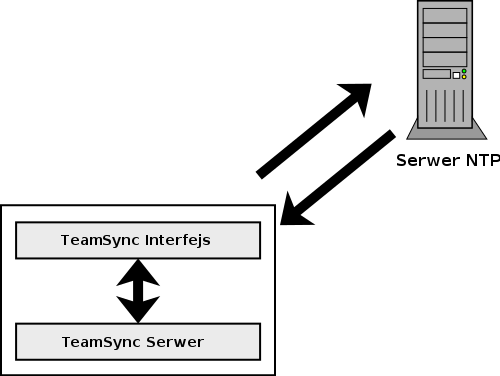
\includegraphics[width=230pt]{figures/architecturentp.png}
  \end{center}
  \caption{Komunikacja systemu \emph{TeamSync} z serwerem NTP.}
\end{figure}

Istnienie możliwości zamieszczania komentarzy przez użytkowników w dowolnej chwili działania systemu \emph{TeamSync} oraz konieczność zachowania informacji o czasie wprowadzania wypowiedzi są źródłami kilku problemów. Chcąc umożliwić rzetelne --- nie tylko co do treści, ale również co do czasu zamieszczenia komentarza --- dzielenie się swoimi opiniami przez użytkowników, należało uniknąć w systemie dwóch nastepujących przeszkód:

\begin{itemize}[noitemsep]
  \item nie ma pewności, że na każdym z węzłów jest ten sam czas systemowy, z którego użytkownik pobierałby znacznik czasowy podczas umieszczania komentarza. Jeśli różnica między czasami zamieszczanych komentarzy byłaby większa niż kilka minut, wyświetlane wypowiedzi często byłyby przedstawiane w nieprawidłowej kolejności. Komentarze napisane później (według czasu rzeczywistego) --- w wyniku różnic czasów systemowych na węzłach --- mogłyby zostać umieszczone w sieci jako napisane wcześniej niż w rzeczywistości,
  
  \item nie ma gwarancji, że wszystkie węzły w jednolity sposób będą wprowadzać znaczniki czasowe do systemu --- problem użytej przez nich jednostki oraz formatu.
\end{itemize}

\emph{Serwer NTP} \cite{ntp}, od którego użytkownicy pobierają znaczniki czasowe podczas zamieszczania komentarzy, pełni rolę neutralnego arbitra i zarazem stanowi rozwiązanie dwóch powyższych zastrzeżeń. Otrzymywanie znaczników czasowych z tego samego dla wszystkich użytkowników, neutralnego źródła jest kluczowym punktem w algorytmie dodawania nowych wypowiedzi --- w przypadku jego braku, użytkownicy mogliby wprowadzać do sieci fałszywe dane.

Potrzeba zachowania jednolitego formatu oraz jednostki znacznika czasowego wynika z konieczności zapewnienia unikalności nazw plików zawierających dane z komentarzami. Bez dostępu do serwera NTP użytkownik nie ma możliwości napisać wypowiedzi w żadnym z wątków, ponieważ narażałoby to system na generowanie konfliktów (np. poprzez dwukrotne uzyskanie tego samego znacznika czasowego przy dodaniu komentarza).

Zapytanie wysyłane jest do serwera NTP \emph{zawsze}, gdy użytkownik umieści treść komentarza (lub nowego wątku) w interfejsie graficznym i zatwierdzi jego dodanie. W odpowiedzi serwer NTP odsyła wiele wartości takich jak: znacznik czasowy, przesunięcie, precyzja, wersja protokołu itd. Najważniejszym z nich (i jedynym użytym w systemie) jest sam znacznik czasowy.

Znacznikiem czasowym, który użytkownicy otrzymują w odpowiedzi jest skoordynowanym czasem uniwersalnym (\emph{UTC --- Universal Coordinated Time}) w postaci liczby całkowitej zawierającą sekundy.